\documentclass[10pt,journal,compsoc]{IEEEtran}
\usepackage[utf8]{inputenc}
\usepackage{amsmath,amsfonts,amssymb}
\usepackage{graphicx}
\usepackage{booktabs}
\usepackage{hyperref}
\usepackage{cite}
\usepackage{listings}
\usepackage{xcolor}

\lstset{
  basicstyle=\ttfamily\footnotesize,
  breaklines=true,
  frame=single,
  backgroundcolor=\color{gray!10}
}

\title{Multi-Agent System for Software Development Lifecycle (SDLC) Automation\\
\large Deliverable 1 (Final): Project Framing, Problem Definition, Data Preprocessing, and Exploratory Analysis}

\author{Hania~Zahra,
        Hamza~Abbas,
        and~Muhammad~Abdullah%
\thanks{All authors contributed equally to the research design, data acquisition pipeline, preprocessing, and exploratory evaluation.}
}

\begin{document}

\maketitle

\begin{abstract}
Modern software development requires orchestrating disjoint specialized disciplines, including requirements engineering, architectural schema modeling, frontend and backend implementation, security auditing, and automated testing. In this report for Deliverable~1, we establish the theoretical framing, problem definition, and empirical data engineering foundation for an autonomous Software Development Lifecycle (SDLC) multi-agent platform. We formulate the limitations of monolithic LLM assistants and justify the requirement for multi-agent machine learning over deterministic, rule-based scaffolding tools. To rigorously benchmark autonomous software development, we construct a 40-scenario benchmark dataset combining 25 curated industry scenarios with 15 real-world GitHub issues across five core software archetypes (CRUD, REST APIs, Authentication, Database-driven applications, and E-commerce). We implement a multi-stage preprocessing pipeline incorporating Interquartile Range (IQR) outlier filtering, categorical One-Hot Encoding, numeric Min-Max scaling, and TF-IDF text vectorization, yielding a 77-dimensional feature space. Finally, we establish a 70/15/15 stratified train/val/test split and provide comprehensive exploratory data analysis (EDA) visualizations demonstrating dataset balance, DAG dependency depth, and agent task distributions.
\end{abstract}

\begin{IEEEkeywords}
Software Development Lifecycle, Multi-Agent Systems, Data Acquisition, Feature Engineering, Exploratory Data Analysis, Benchmark Dataset.
\end{IEEEkeywords}

\section{Phase 1: Project Framing and Problem Definition}

\subsection{Problem Statement}
In modern enterprise software engineering, translating high-level business requirements into deployable, secure, and fully verified full-stack applications is a labor-intensive and error-prone undertaking. While recent advances in foundation Large Language Models (LLMs) have yielded developer assistants for code completion and snippet generation, attempting to automate end-to-end SDLC workflows with a single monolithic LLM prompt introduces critical failure modes:
\begin{enumerate}
    \item \textbf{Context Diffusion and Constraint Loss:} As project prompts expand to encompass multi-file backend routes, frontend state stores, relational database schemas, and configuration files, monolithic LLMs suffer from severe attention diffusion. Non-functional requirements (e.g., database foreign-key constraints, CORS security headers, rate limiting) are routinely omitted.
    \item \textbf{Unchecked Hallucinations and Inconsistent Contracts:} Monolithic architectures operate open-loop without internalized verification gates. Models routinely reference fictitious third-party libraries, generate incompatible data models between the backend API and frontend client, and invent nonexistent endpoints.
    \item \textbf{Absence of Adversarial Persona Specialization:} A single agent context cannot simultaneously adopt the creative, product-oriented perspective of a Product Manager, the structural discipline of a System Architect, and the adversarial paranoia of a Security Auditor.
\end{enumerate}

To resolve these failure modes, we propose an autonomous multi-agent orchestration architecture utilizing LangGraph \cite{langchain2024} and cooperative multi-agent meta-frameworks \cite{hong2023metagpt} to model the software engineering team as a directed cyclic state graph with dedicated human-in-the-loop review gates.

\subsection{Target Audience and Operational Use Cases}
The proposed platform addresses three primary target audiences:
\begin{itemize}
    \item \textbf{Agile Engineering Teams and Technical Leads:} Rapidly bootstrapping fully functional, production-ready full-stack prototypes from Jira issue tickets, complete with OpenAPI contracts, relational schemas, unit tests, and Docker deployment configurations.
    \item \textbf{Full-Stack Developers:} Automating the repetitive, error-prone scaffolding of REST endpoints, SQLAlchemy models, Pydantic validation schemas, and Next.js frontend pages while preserving architectural consistency.
    \item \textbf{DevOps and Quality Assurance Engineers:} Eliminating manual test scaffolding and security auditing by autonomously generating unit test suites and executing static vulnerability scans prior to deployment.
\end{itemize}

\subsection{AI Justification: Machine Learning vs. Traditional Rule-Based Approaches}
Traditional software scaffolding solutions (e.g., Yeoman, cookiecutter, Rails generators) rely on rigid, deterministic code templates and static syntax trees. While these deterministic tools excel at generating uniform directory structures, they exhibit fundamental limitations:
\begin{itemize}
    \item \textbf{Inability to Comprehend Ambiguous Natural Language:} Deterministic engines cannot interpret nuanced business specifications, user stories, or open-ended Jira descriptions.
    \item \textbf{Lack of Cross-Domain Reasoning:} Template engines cannot reason about business domain constraints, synthesize custom relational schema relationships, or construct algorithmic endpoints matching specific user intents.
    \item \textbf{Inflexibility to Error Diagnostics:} When compiler or linting errors occur, deterministic generators cannot inspect runtime stack traces, infer root causes, and autonomously synthesize corrected code diffs.
\end{itemize}

In contrast, deep learning foundation models \cite{touvron2023llama} and retrieval-augmented systems \cite{lewis2020retrieval} possess rich semantic comprehension, probabilistic program synthesis capabilities, and multi-turn conversational reasoning. By structuring foundation models into specialized agents with scoped memory, dedicated toolsets, and closed-loop feedback mechanisms, our framework balances autonomous semantic synthesis with deterministic compiler verification.

\section{Phase 2: Data Acquisition and Preprocessing Pipeline}

\subsection{Benchmark Data Collection}
To evaluate both single-agent baselines and multi-agent architectures on standardized tasks, we curated a 40-scenario benchmark dataset. As documented in Table~\ref{tab:dataset_composition}, the dataset balances two complementary sources:
\begin{itemize}
    \item \textbf{Curated Industry Scenarios ($N=25$):} Authored to represent common enterprise full-stack development patterns across diverse architectural complexities, specifying functional user stories, data schemas, API routes, and planted security vulnerabilities.
    \item \textbf{Real-World GitHub Issues ($N=15$):} Extracted and curated from high-impact open-source repositories using GitHub's REST API. These scenarios reflect real-world developer language, implicit environmental dependencies, and authentic defect reports.
\end{itemize}

\begin{table}[h]
\centering
\caption{Benchmark Dataset Archetype Composition}
\label{tab:dataset_composition}
\begin{tabular}{lcccc}
\toprule
\textbf{Software Archetype} & \textbf{Manual} & \textbf{GitHub} & \textbf{Total} & \textbf{Ratio (\%)} \\
\midrule
CRUD Operations & 5 & 3 & 8 & 20.0\% \\
REST API Services & 5 & 3 & 8 & 20.0\% \\
Authentication Subsystems & 5 & 3 & 8 & 20.0\% \\
Database Applications & 5 & 3 & 8 & 20.0\% \\
E-Commerce Backends & 5 & 3 & 8 & 20.0\% \\
\midrule
\textbf{Total Benchmark} & \textbf{25} & \textbf{15} & \textbf{40} & \textbf{100.0\%} \\
\bottomrule
\end{tabular}
\end{table}

\subsection{Data Cleaning and Outlier Detection}
To ensure robust benchmark evaluation, raw scenario inputs underwent rigorous programmatic validation:
\begin{itemize}
    \item \textbf{Schema Validation and Null Handling:} Every scenario is validated against a Pydantic schema enforcing required keys: category, functional requirements list, entity schema, API endpoints, and planted CWE vulnerability definitions. Missing optional fields were deterministically imputed.
    \item \textbf{Deduplication:} Exact and normalized text deduplication was applied to prevent duplicate prompt injection across splits.
    \item \textbf{Interquartile Range (IQR) Outlier Detection:} We analyzed character lengths across all scenario requirements prompts. Let $Q_1$ and $Q_3$ represent the first and third quartiles. The bounds were computed as:
    \begin{equation}
    [\text{Lower}, \text{Upper}] = [Q_1 - 1.5 \times \text{IQR}, \; Q_3 + 1.5 \times \text{IQR}]
    \end{equation}
    Character lengths ranged from 263 to 330 characters (mean = 292 characters), with zero outliers detected beyond the $[1.5 \times \text{IQR}]$ thresholds, confirming tight, consistent benchmark prompt formatting.
\end{itemize}

\subsection{Feature Engineering and Representation Strategy}
To enable quantitative clustering, difficulty estimation, and baseline classification, we engineered a 77-dimensional tabular feature representation:
\begin{enumerate}
    \item \textbf{Categorical One-Hot Encoding (7 features):} One-hot encodings for the five application categories (\texttt{category\_auth}, \texttt{category\_crud}, \texttt{category\_db\_app}, \texttt{category\_ecommerce}, \texttt{category\_rest\_api}) and two data origins (\texttt{source\_github}, \texttt{source\_manual}).
    \item \textbf{Continuous Numeric Scaling (6 features):} Min-Max scaling normalized into $[0, 1]$ over six scenario structural complexity attributes: character length, word count, functional requirement count, decomposition task count, maximum DAG dependency depth, and security requirement count.
    \item \textbf{TF-IDF Text Representations (64 features):} Term Frequency-Inverse Document Frequency vectorizer extracted over requirement descriptions using unigram and bigram tokens with sublinear term-frequency scaling.
\end{enumerate}

\subsection{Dataset Stratification Strategy}
To guarantee representative evaluation across all lifecycle stages, the 40 scenarios were partitioned using stratified random sampling into:
\begin{itemize}
    \item \textbf{Development Split (70\%, $N=28$):} Used for prompt tuning, agent role calibration, and tool interface design.
    \item \textbf{Validation Split (15\%, $N=6$):} Dedicated to hyperparameter grid search (temperature, max review loops, retrieval top-$k$).
    \item \textbf{Holdout Test Split (15\%, $N=6$):} Strictly sequestered for unbiased final empirical evaluation of both the baseline and multi-agent systems.
\end{itemize}
Stratification strictly maintained the 20\% category representation across all three splits.

\begin{figure}[t]
\centering
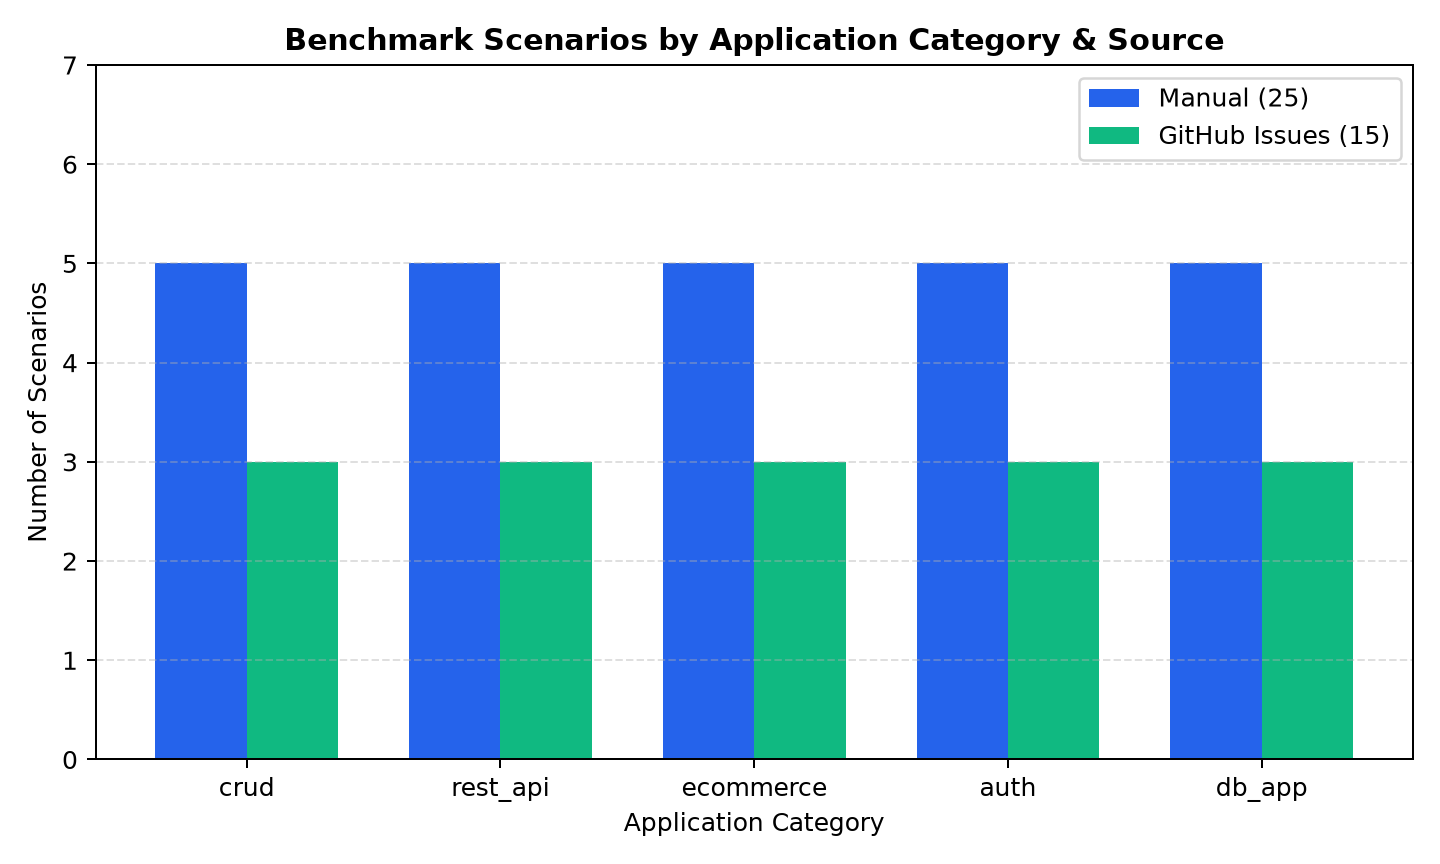
\includegraphics[width=\linewidth]{../reports/figures/category_source_distribution.png}
\caption{Scenario Category and Source Origin Distribution across the 40 Benchmark Scenarios.}
\label{fig:category_source}
\end{figure}

\begin{figure}[t]
\centering
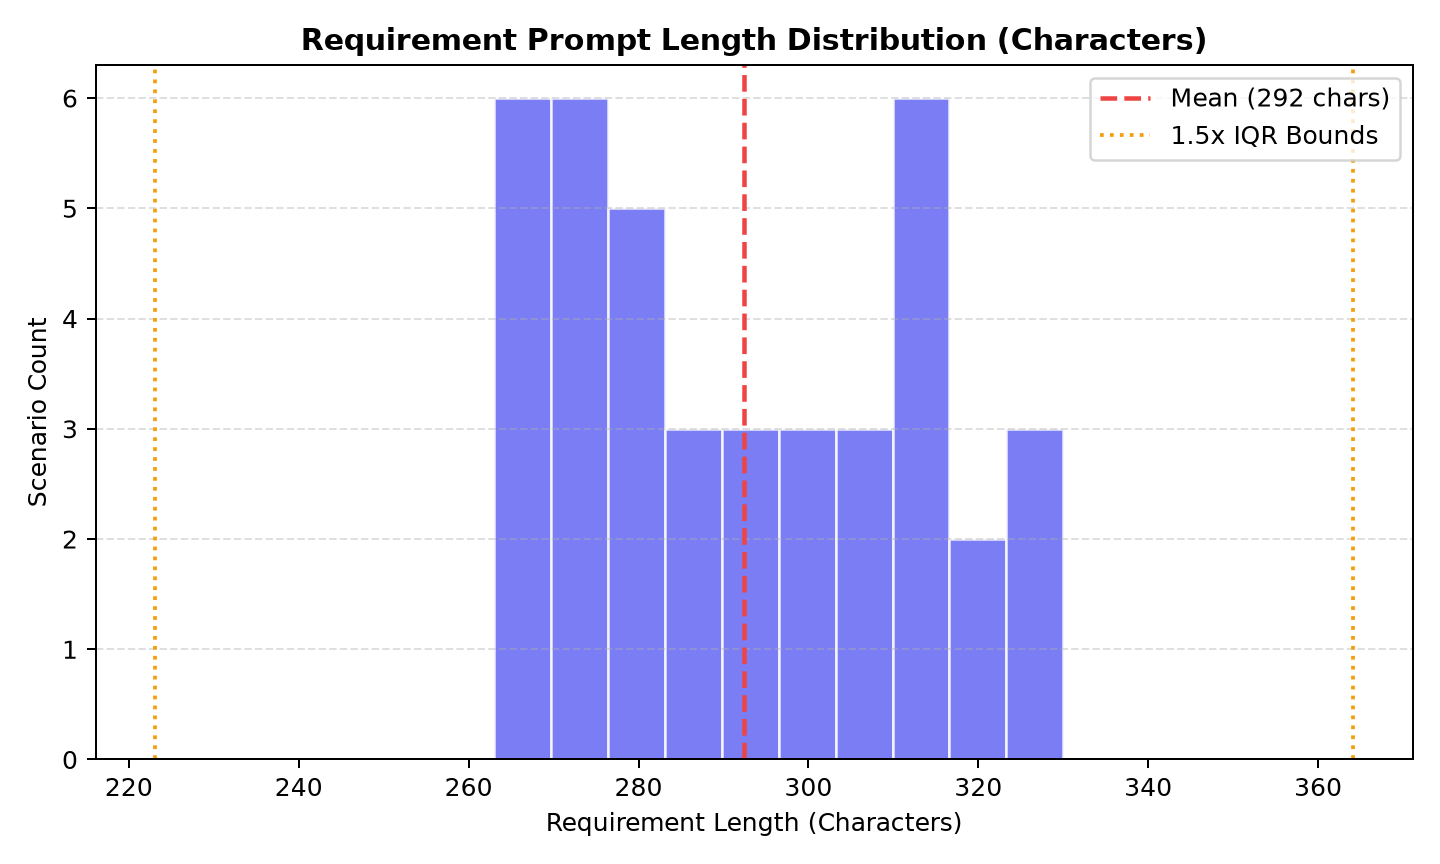
\includegraphics[width=\linewidth]{../reports/figures/requirement_length_distribution.png}
\caption{Prompt Character Length Distribution across Benchmark Scenarios (Min = 263, Max = 330, Mean = 292 characters).}
\label{fig:req_length}
\end{figure}

\begin{figure}[t]
\centering
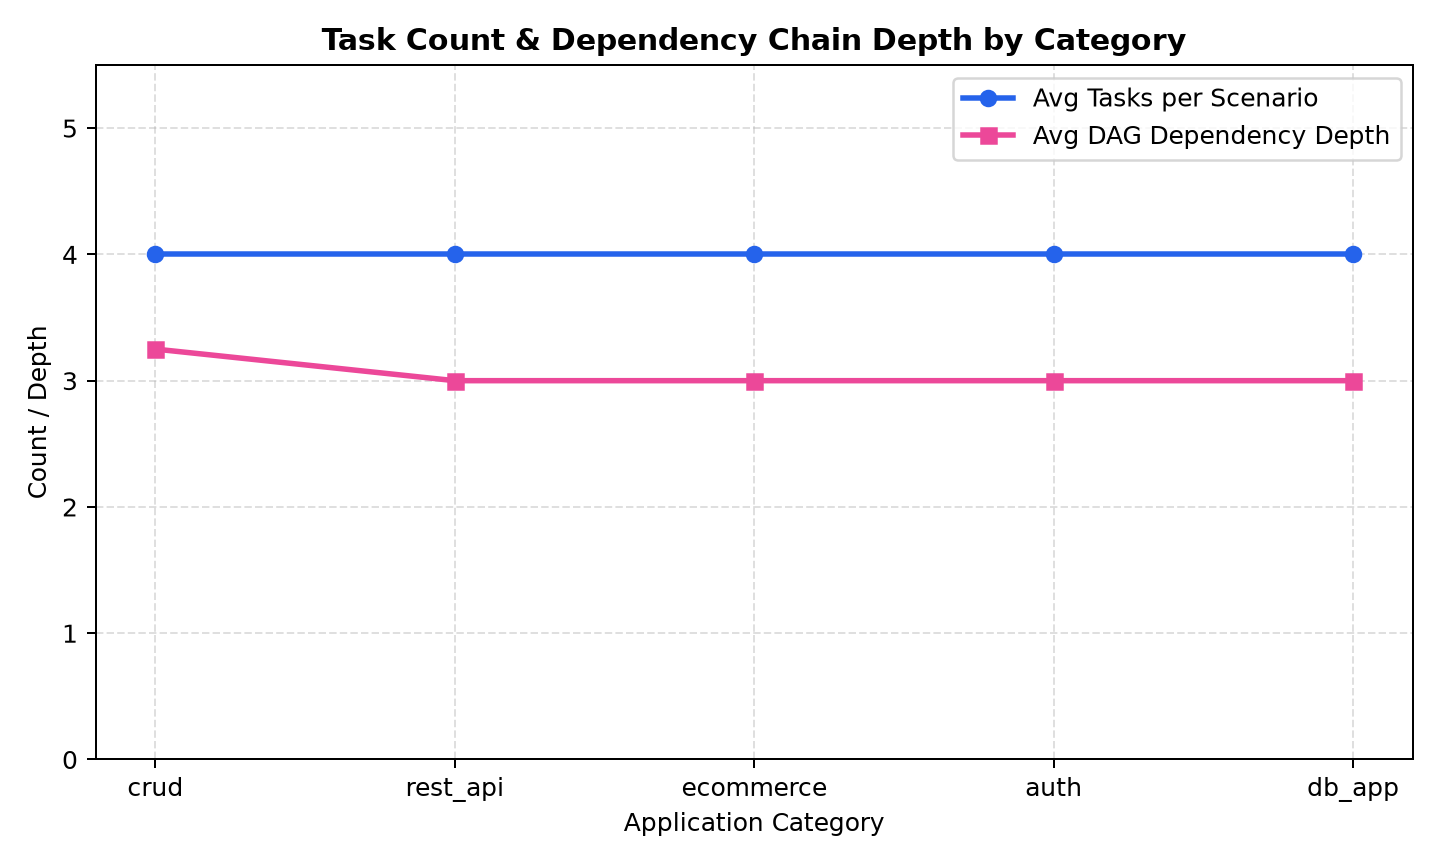
\includegraphics[width=\linewidth]{../reports/figures/dependency_depth_distribution.png}
\caption{Task DAG Maximum Dependency Depth Distribution across Benchmark Scenarios.}
\label{fig:dag_depth}
\end{figure}

\begin{figure}[t]
\centering
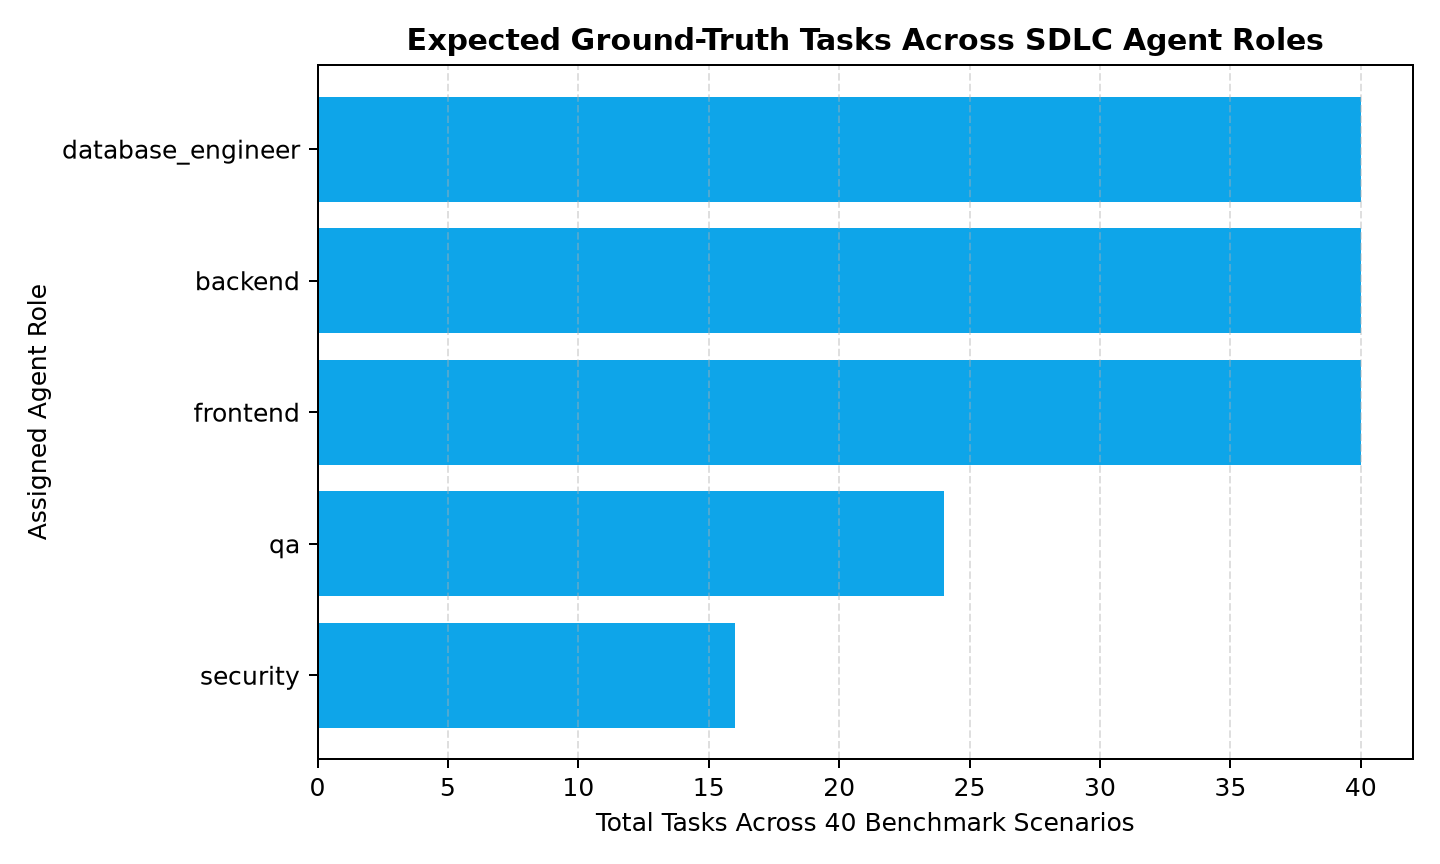
\includegraphics[width=\linewidth]{../reports/figures/tasks_by_agent_role.png}
\caption{Distribution of Synthesized Development Sub-tasks Partitioned by Specialist Agent Role.}
\label{fig:tasks_by_role}
\end{figure}

\section{Phase 2: Exploratory Data Analysis (EDA)}

Comprehensive visual exploratory analysis was conducted across the preprocessed benchmark dataset:
\begin{itemize}
    \item \textbf{Category and Source Distribution:} As illustrated in Figure~\ref{fig:category_source}, each of the five architectural categories comprises exactly 8 scenarios (20\% each), with 5 manual scenarios and 3 mined GitHub scenarios per category. This uniform distribution prevents categorical bias in downstream agent evaluation.
    \item \textbf{Requirement Length Distribution:} Figure~\ref{fig:req_length} shows the unimodal, compact distribution of prompt character lengths, centered at 292 characters, verifying that all scenarios provide concise, actionable specifications without excessive verbosity.
    \item \textbf{DAG Dependency Depth:} Figure~\ref{fig:dag_depth} examines the maximum topological depth of the synthesized task dependency graphs. The majority of scenarios exhibit a dependency depth between 3 and 4 levels (e.g., Schema Definition $\rightarrow$ Database Migration $\rightarrow$ Backend Route $\rightarrow$ Frontend UI $\rightarrow$ QA Validation), establishing non-trivial dependency chains that require topological scheduling.
    \item \textbf{Agent Task Allocation:} Figure~\ref{fig:tasks_by_role} breaks down subtasks assigned to domain specialist agents. Backend and Database tasks represent the largest volume of generated tasks, followed by Frontend, Reviewer, QA, and Security verification tasks.
\end{itemize}


\section{Link to the Evaluation (Final Status)}
The 40-scenario benchmark and its 70/15/15 split were used unchanged in Deliverable~2. The live evaluation covered all six held-out test scenarios (\texttt{scen\_003}, \texttt{scen\_008}, \texttt{scen\_012}, \texttt{scen\_020}, \texttt{scen\_024}, \texttt{scen\_037}) and two validation scenarios (\texttt{scen\_005} completed, \texttt{scen\_014} run and analyzed as a failure case). The completed scenarios span the CRUD, REST API, E-commerce, Authentication, and Database-application archetypes; every scenario in the evaluated set has medium complexity. Because only a subset of the benchmark was executed (seven completed runs out of 40 scenarios), results should be read as a case study and not as a statistically powered evaluation.
\section{Deliverable 1 Team Contribution Statement}
Table~\ref{tab:d1_contributions} details team member contributions during Deliverable~1.

\begin{table*}[t]
\centering
\caption{Team Member Contributions for Deliverable 1}
\label{tab:d1_contributions}
\resizebox{\textwidth}{!}{
\begin{tabular}{lp{3.5cm}cp{10.2cm}}
\toprule
\textbf{Member} & \textbf{Role} & \textbf{Commits} & \textbf{Specific Deliverable 1 Subsystem Contributions} \\
\midrule
Hamza Abbas & Architecture Lead & 5 & Problem formulation, target audience scoping, AI justification, baseline architecture design, repository configuration, and git workflow setup. \\
\addlinespace
Muhammad Abdullah & Data Engineer & 4 & GitHub Issues REST API mining script (\texttt{collect\_github\_issues.py}), data ingestion pipeline, feature engineering strategy (One-Hot, MinMax, TF-IDF), and dataset building automation. \\
\addlinespace
Hania Zahra & Evaluation Lead & 4 & Authoring 25 manual benchmark scenarios, data cleaning and validation scripts (\texttt{clean.py}), IQR outlier detection, stratified train/val/test split execution, and EDA visualization generation. \\
\midrule
\textbf{Total} & & \textbf{13} & \textbf{Phase 1 Framing \& Phase 2 Complete Data Engineering Pipeline} \\
\bottomrule
\end{tabular}
}
\end{table*}

\bibliographystyle{IEEEtran}
\bibliography{references}

\end{document}
